\setcounter{secnumdepth}{1}
\section{Einführung}
Diese Bachelorarbeit behandelt die Ausführung und Verarbeitung von asynchronen Prozessen in der Programmierung speziell in der Sprache Typescript.\\

\noindent
Zielgruppe dieser Arbeit sind Personen, die Grundkenntnisse in der Sprache Javascript/Typescript vorweisen können.
Sollte man von der Skriptsprache Typescript noch nie/kaum etwas gehört haben, sollte vor dem Lesen dieser Arbeit die offizielle Dokumentation von Microsoft durchgegangen werden.

\begin{center}
\url{https://www.typescriptlang.org/docs/home.html} 
\end{center}

\noindent
In dieser Arbeit wird nur oberflächlich auf die Unterschiede der beiden Sprachen eingegangen. Des Weiteren sollte man von den Kernkonzepten der Promises und Observables schon mal gehört haben, da diese in der Arbeit gegenübergestellt werden.

\subsection{Typescript}
Typescript. Bereits der Name sagt schon was diese Sprache ausmacht. Sie \textit{(\glqq{}Type\grqq{} zu deutsch: Typ)} ist eine typisierte Form der Skriptsprache Javascript. In Typescript ist es Standard, jede Variable, Funktion und Funktionsparameter im Vorfeld zu typisieren. Mit dem Typescript Compiler werden Dateien mit dem Suffix *.ts in *.js überführt.

\subsubsection{Beispiel}

\begin{figure}[h!]
\begin{lstlisting}
class Greeter {
    greeting: string;
    constructor (message: string) {
        this.greeting = message;
    }
    greet() {
        return "Hello, " + this.greeting;
    }
}  
\end{lstlisting}
\caption{Typescript Klasse \cite{typescript-example}}
\end{figure}

\noindent
Im oberen Code-Schnipsel wurden die variablen und die Klassenmethoden nach Typescript-Standard deklariert. Diese Typen werden beim übersetzen in Javascript ignoriert. Der Kompiler einer Entwicklungsumgebung prüft dann, ob beim übergeben eines Parameters in den Konstruktor ein numerischer oder Boolean-Wert eingesetzt wird. Dies wird dann als ein Fehler erkannt. Der Kompiler übersetzt auch nicht direkt deklarierte Typen. Wie in diesem Fall wird erkannt, dass die Methode greet() einen String-Wert zurückgibt.

\begin{figure}[t]
\begin{lstlisting}
var Greeter = (function () {
    function Greeter(message) {
        this.greeting = message;
    }
    Greeter.prototype.greet = function () {
        return "Hello, " + this.greeting;
    };
    return Greeter;
})(); 
\end{lstlisting}
\caption{Überführung in Javascript \cite{typescript-example}}
\end{figure}

\noindent
In der vom Kompiler auf Javascript übersetzten Version werden die erstellten Klassen und Typen vollständig eliminiert. Was verbleibt ist die Übersetzung der Klassen-Methode greet() und des Konstruktors. Sowohl Klassen (erst ab ECMAScript2015 verfügbar) als auch Interfaces werden in Javascript nicht genutzt.

\subsubsection{Kompiler}
In einer tsconfig.json Datei können die Kompiler-Optionen für Typescript gesetzt werden. Zudem können Root-Dateien definiert und ausgeschlossen werden. Die Auflistung einer tsconfig.json Datei in einem Verzeichnis zeigt, dass es sich hierbei um das Root-Verzeichnis des Projekts handelt. Ein Beispiel für die Konfiguration einer solchen Datei könnte wie folgt aussehen: 

\begin{figure}[h!]
\begin{lstlisting}
{
    "compilerOptions": {
        "module": "system",
        "noImplicitAny": true,
        "removeComments": true,
        "preserveConstEnums": true,
        "outFile": "../../built/local/tsc.js",
        "sourceMap": true
    },
    "include": [
        "src/**/*"
    ],
    "exclude": [
        "node_modules",
        "**/*.spec.ts"
    ]
}  
\end{lstlisting}
\caption{tsconfig.json \cite{tsconfig}}
\end{figure}

\noindent
Hier kann z.B. mit der Regel \glqq noImplicitAny\grqq{} festgelegt werden, dass Methoden als auch Parameter und Variablen getypt werden müssen bei ihrer Deklaration. Sind sie nicht getypt: Bedeutet dies für den Kompiler sie sind als any deklariert.
\noindent
Die Konfiguration dieser Datei betrifft Kompilier-Fehler. Fehler zur Laufzeit sind von der Konfiguration ausgeschlossen. Zudem wird in jedem Fall eine Javascript-Datei erstellt, auch wenn der Kompiler einen Fehler anzeigt. Diese Datei ist potenziell auch lauffähig.\\\\
\noindent
Da Syntaktisch alles was auf Javascript geschrieben wird, auch valider Typescript Code ist, kann man Typescript als Superset von Javascript bezeichnen. Demzufolge kann man die Nutzung von statische Typen, Klassen und Interfaces als Konvention betrachten.

\subsubsection{Entwicklung}
Im Laufe der Zeit findet Typescript immer mehr Beliebtheit in Unternehmensprojekten. Entwicklerteams können durch die Typisierung schneller Bugs am Code erkennen und durch den modularen Aufbau, den Typescript ermöglicht, die Organisation und Dokumentation von großen Projekten verbessern. Diese Tendenz wird von der Entwicklerplattform Stackoverflow untermauert, die in einer Umfrage die beliebtesten Programmiersprachen der Entwickler prüfte.
Dabei ist folgendes rausgekommen:

\begin{figure}[H]
\centering
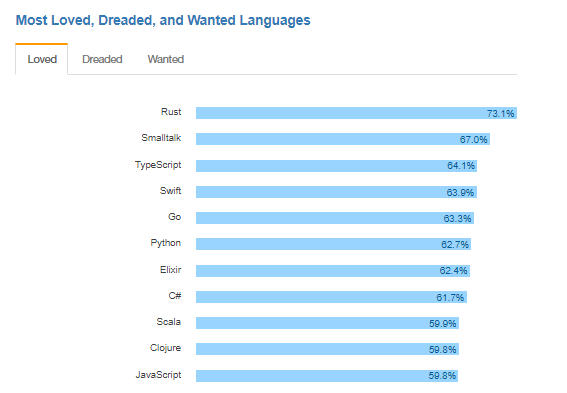
\includegraphics[height=6cm]{stackoverflow-typescript-popularity}
\caption{Prozentualer Anteil der Entwickler die Interesse an neuen Technologien zeigen und weiter mit neuen Technologien arbeiten möchten. Jahr: 2017 \cite{typescript-survey}}
\end{figure}

\subsection{Aufbau}
Diese Bachelorarbeit wird aus zwei Code-Projekten bestehen. Während das erste Projekt nur im Kern die Ausführung von asynchronen Verarbeitungsprozessen präsentiert (mit der Hilfe von simulierten Anwendungsbeispielen), wird das zweite Projekt eine Singlepage-Applikation darstellen und praxisnahe Beispiele anwenden. Dies soll mit dem Framework Angular und Google Firebase als DaaS bewerkstelligt werden. Das zweite Projekt wird im zweiten Teil der Arbeit näher vorgestellt. Die Repositories für beide Projekte sind zu finden unter: 

\begin{center}
\url{https://github.com/MarcoLeko/Promises-vs.-Observables.git} \\
\url{https://github.com/MarcoLeko/Angular-Firebase-App.git}
\end{center}

\noindent
Zu beachten ist, dass vor dem Ausführen beider Projekte \textbf{Node.js} auf dem Rechner installiert sein muss, um den integrierten Paket-Manager \textbf{npm} nutzen zu können. Da rxjs nicht von vornherein von Javascript mitgeliefert wird, wird eine sog. \glqq  Third-Party Library\grqq{} dafür benötigt. Daraufhin muss in dem Root-Verzeichnis beider Projekte \textbf{npm install} ausgeführt werden, um die jeweiligen Abhängigkeiten dieser Libraries herunterzuladen. Node.js kann man unter folgendem Link herunterladen:

\begin{center}
\url{https://nodejs.org/en/}
\end{center}

\subsection{Zielsetzung}
Ziel der Arbeit ist die Betrachtung und Aufbereitung des Einsatzes von Sprachmitteln zur asynchronen Verarbeitung in Typescript in einer Form, die Einsteigern in die Thematik hilft, die unterschiedlichen Konzepte voneinander abzugrenzen und richtig einzusetzen. Dazu soll asynchrone Verarbeitung insgesamt anhand brauchbarer und für den Einsatz von Typescript typischer Szenarien motiviert werden. Es werden die zur Verfügung stehenden Sprachmittel Promises und Observables mit ihren jeweiligen Features vorgestellt. Dabei soll nach dem Vorstellen der beiden Kernkonzepte im zweiten Teil der Arbeit \glqq Best Practice\grqq{}-Beispiele vorgeführt werden. Nach dem Lesen dieser Arbeit soll der Leser ein gewisses Verständnis dafür gewonnen haben, welche der vorgestellten Sprachmitteln für welchen Anwendungsfall sinnvoller erscheint. 

\subsection{Terminologie}
Um die Abgrenzung von verschiedenen asynchronen Sprachmitteln zu beherrschen, muss vorerst geklärt werden, was Asynchronität bedeutet.

\subsubsection{Einführung}
Der zentrale Teil eines Computers, welches Programme und einzelne Schritte zum Ausführen bringt, ist der Prozessor. Die Geschwindigkeit in der eine Schleife von einem Programm ausgeführt wird, hängt von der Geschwindigkeit des Prozessors ab. Programme interagieren jedoch mit Operationen außerhalb des Zuständigkeitsbereiches eines Prozessors, wie z.B. die Kommunikation über ein Netzwerk oder Abfragen von Daten von der Festplatte. Solche Operationen hängen von anderen Ressourcen ab und brauchen Zeit. In solchen Szenarien wäre es unvorteilhaft, wenn der Prozessor, anstatt andere Operationen in der Zwischenzeit auszuführen, im Leerlauf stecken würde. Genau für solche Aufgaben ist das Betriebssystem da. Das Betriebssystem sorgt dafür, dass Kapazitäten des Prozessors auf parallel laufende Programme wechselt, während es auf die Antwort von ausgeführten Operationen wartet. Es entstehen dabei verschiedene \glqq Threads\grqq{}. Und hier kommt die Asynchronität ins Spiel:

\subsubsection{Asynchronität}
Ein \textbf{asynchrones} Programmiermodell erlaubt multiple Abläufe zum selben Zeitpunkt. Wenn eine Aktion ausgeführt wird, läuft das Programm in einem anderen \glqq Thread\grqq{} weiter. Sollte die Operation fertig gestellt sein, wird das Programm informiert und liefert das Ergebnis zurück. Ein Beispiel dafür wäre das Suchen von Dateien auf einer Festplatte.\cite{asynchronitaet} \\

\subsubsection{Synchronität}
In einem \textbf{synchronen} Programmiermodell entstehen Abläufe sequenziell. Wenn eine Funktion mit einer zeitintensiven Aktion abgerufen wird, wird das Ergebnis erst nach dem Beenden der Operation zurückgegeben. In diesem Zeitintervall werden keine Nebenoperationen ausgeführt.\cite{asynchronitaet} \\

\subsubsection{Beispiel}
Die Wiedergabe mehrerer Meldungen in einem Browser:

\begin{figure}[H]
\begin{lstlisting}
export class Notifications {

    public msg(msg: string): void {
        document.body.innerHTML +=
            `<div class="alert" role="alert">${msg}</div>` as string;
    }
}

class Synchronous extends Notifications {

    private printMessages(): void {
        this.msg('Hey Im message Nr. 1!');
        this.msg('Hey Im message Nr. 2 !');
        this.msg('Hey Im message Nr. 3 !');
    }

    public printAndTrackTime() {
        const begin = window.performance.now();
        this.printMessages();
        const end = window.performance.now();
        document.body.innerHTML += `<div class="time-box sync">Synchronous: ${end - begin}ms</div>`;
    }
}

class Asynchronous extends Notifications {

    private printMessages(): void {
        this.msg('Hey Im message Nr. 1 !');
        setTimeout(() => this.msg('Hey Im message Nr. 2 !'), 50);
        this.msg('Hey Im message Nr. 3!');
    }

    public printAndTrackTime() {
        const begin = window.performance.now();
        this.printMessages();
        const end = window.performance.now();
        document.body.innerHTML += `<div class="time-box async">Asynchronous: ${end - begin}ms</div>`;
    }
}

const sync = new Synchronous();
const async = new Asynchronous();

sync.printAndTrackTime();
document.body.innerHTML += '<hr>';
async.printAndTrackTime();
\end{lstlisting}
\caption{sync-vs.-async.ts}
\end{figure}

\noindent
Diese Datei enthält drei Klassen. Während \textbf{Notifications} als Basisklasse eine Methode für das Addieren einer Nachricht in die HTML-Dom bereitstellt, rufen die abgeleiteten Klassen \textbf{Synchronous} und \textbf{Asynchronous} die Nachricht in verschiedener Weise auf. In der Klasse Synchronous werden die HTML-Elemente sequenziell in die Dom eingefügt. In der Asynchronous Klasse dagegen wird nur die erste und dritte Nachricht sequenziell ausgeführt. Die zweite Nachricht wird mit einer Verzögerung von 50 Millisekunden in einem neuen Zeitfenster veranlasst. Ein neuer Thread entsteht. Währenddessen wird schon die nächste Operation ausgeführt. Um die Zeit zurückzuverfolgen wurde ein Timer vor der Anzeige der HTML-Elemente gestartet. Dieser wird gestoppt sobald alle Nachrichten innerhalb dieser Methode aufgerufen wurden. Auffallend ist, dass die Methode in der synchronen Ausführung stets länger braucht als die asynchrone Ausführung. Das liegt daran, dass in der asynchronen Ausführung die Zeit nach dem Ausführen der dritten Nachricht und vor dem Ausführen der zweiten Nachricht gestoppt wird, da die zweite Nachricht sich in einem anderen Zeitfenster befindet. Somit wartet der Timer im asynchronen Modell immer nur auf zwei Nachrichten, während das synchrone Modell auf drei Nachrichten wartet.
Das Ergebnis sieht wie folgt aus:

\begin{figure}[H]
\centering
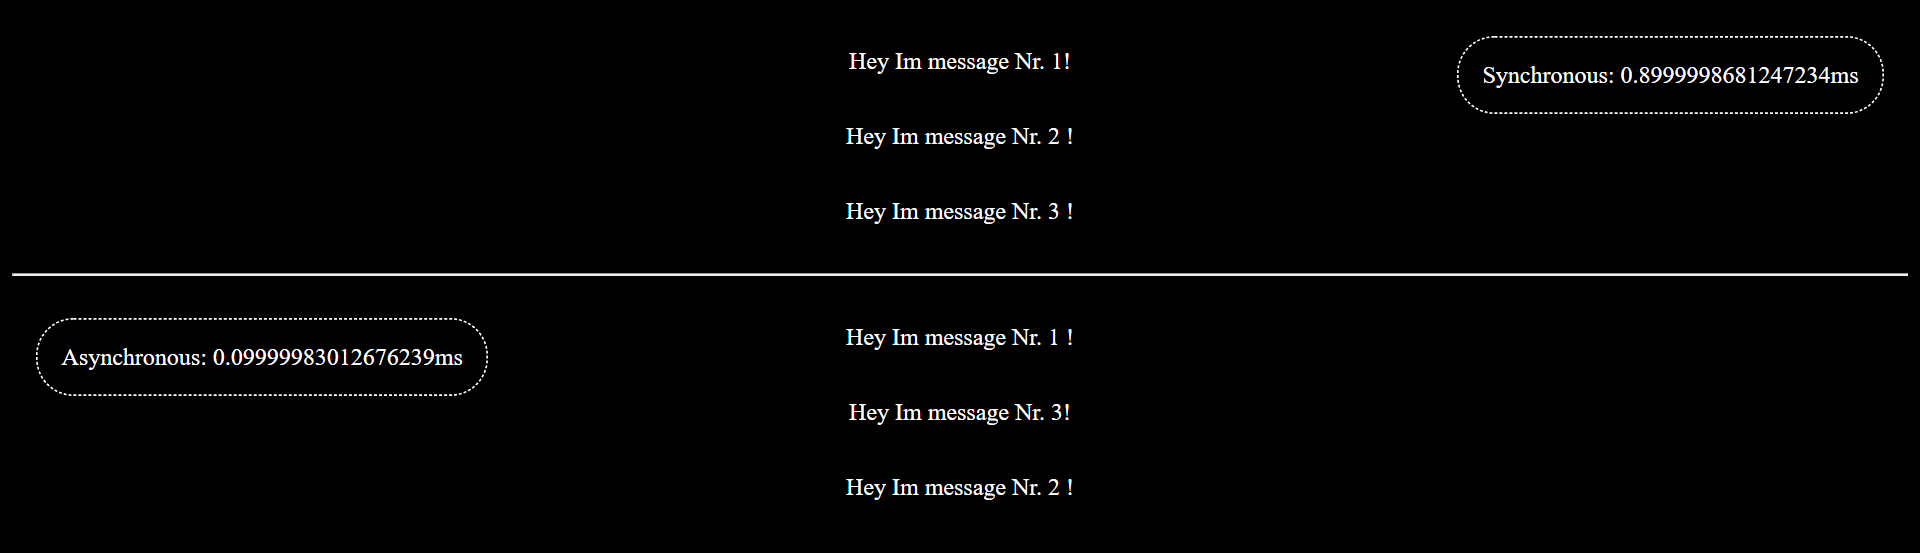
\includegraphics[width=12cm, height=4cm]{synchronous-vs-asynchronous}
\caption{Die Asynchronous Klasse gibt Nachricht 3 aus bevor Nachricht 2 ausgegeben wird.}
\end{figure}

\noindent
Vor dem Ausführen des Beispiels muss folgend konfiguriert werden:
 \begin{center}
     Promises-vs.-Observables$\,\to\,$ webpack.config.js
 \end{center}

\begin{figure}[h!]
\begin{lstlisting}
module.exports = {
    mode: 'development',
    entry: './src/modules/sync-vs-async.ts',
    ...
}
\end{lstlisting}
\caption{Hier sollte die Typescript Datei sync-vs-async.ts als Eingangspunkt definiert werden.}
\end{figure}

\noindent
Nun kann man mit dem Befehl \textbf{npm run start} die Eingangsdatei gebündelt werden. Webpack kompiliert alle importierten Module dieser Datei und erstellt eine zentrale Endversion vom Kompilat in Javascript-Format. Anschließend muss nur noch die HTML-Seite geöffnet werden. \\

\noindent
Zusammenfassend kann man also sagen, dass in dem synchronen Modell implizit auf die Aktionen gewartet wird, und in dem asynchronen Modell explizit. Als Diagramm abgebildet führt der Browser die Methoden wie folgt aus:

\begin{center}
\begin{figure}[H]
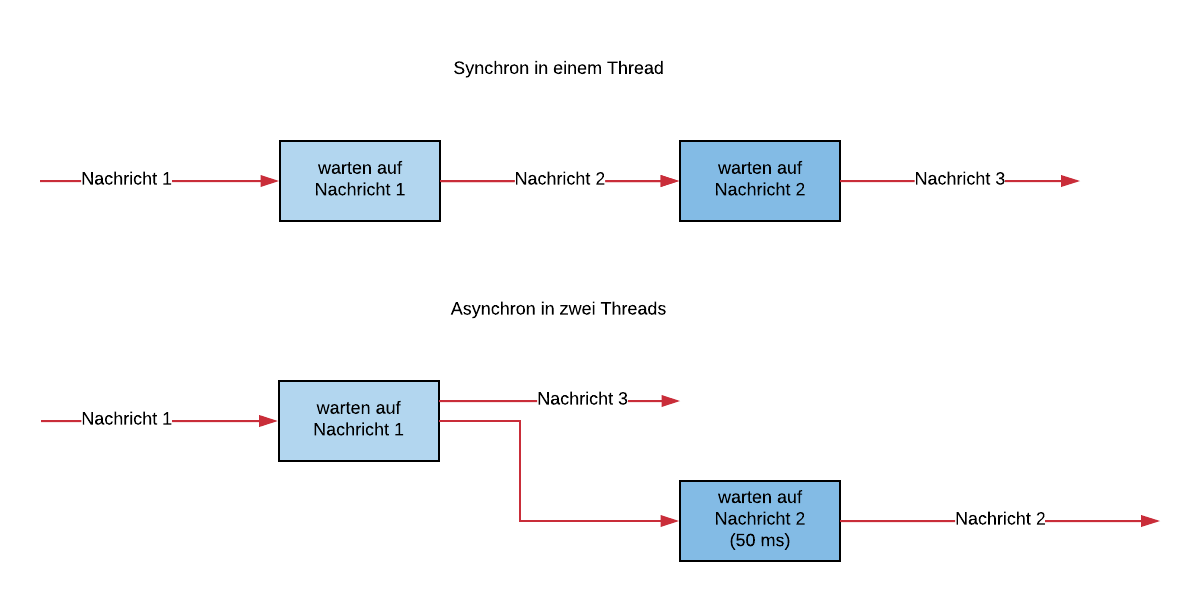
\includegraphics[width=12cm]{synchron-vs-asynchron-diagramm}
\caption{Rot: Browser führt die Methode aus - Blau: Browser wartet}
\end{figure}
\end{center}

\noindent
Das angeführte Beispiel hat mit der Funktion setTimeout eine asynchrone Operation ausgeführt. Funktionen die als Parameter andere Funktionen übergeben werden, nennt man auch \textbf{callback function} - Rückruffunktionen. Es gibt jedoch auch andere Ansätze der asynchronen Prozessverarbeitung. Diese sind unter anderem \textbf{Promises}.





